\documentclass[border=10pt]{standalone}
\usepackage[svgnames]{xcolor}
\usepackage{amsmath}
\usepackage{pgfplots}
\pgfplotsset{compat=newest}
\usepackage[sfdefault]{FiraSans}
\usepackage{FiraMono}
\renewcommand*\familydefault{\sfdefault}
\begin{document}
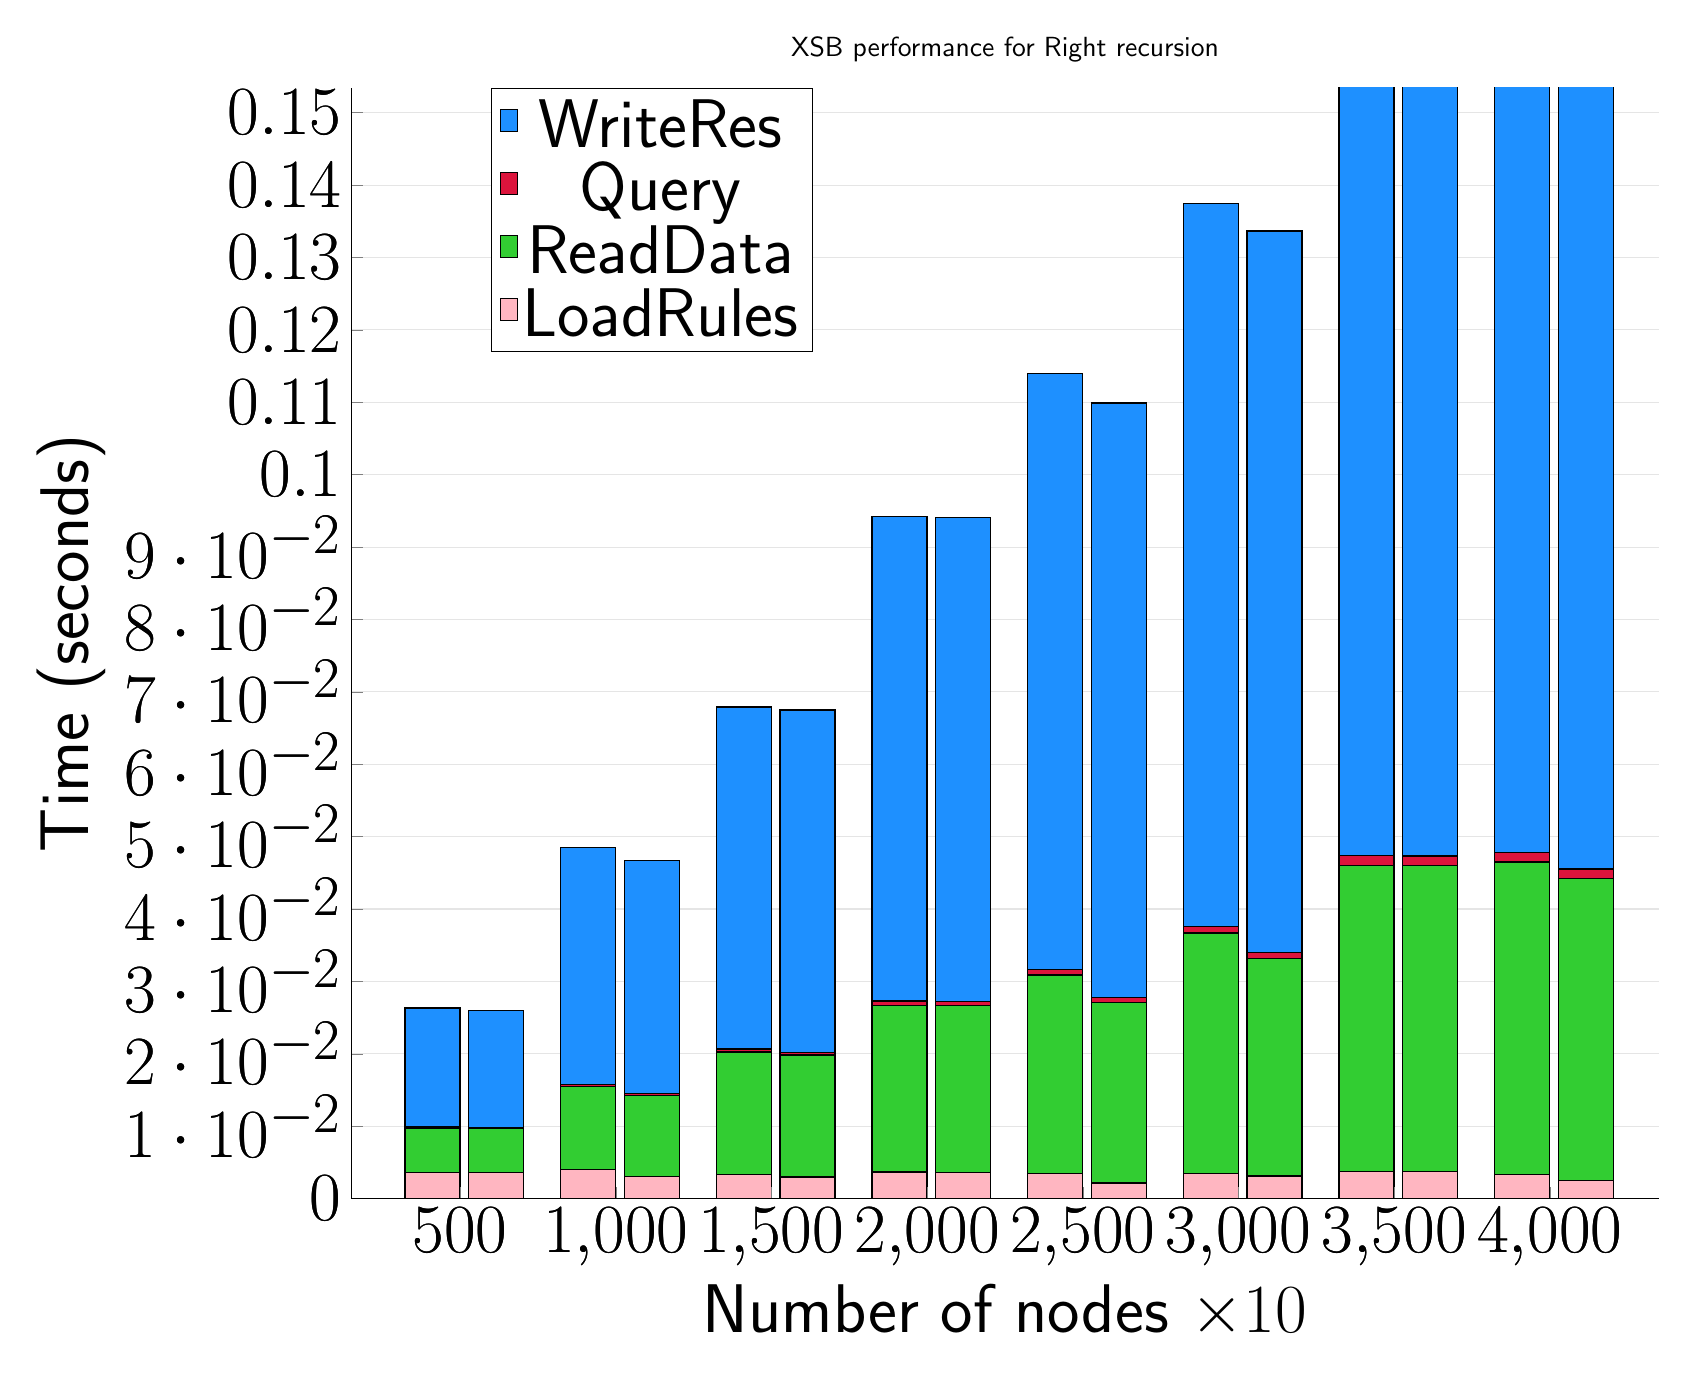
\begin{tikzpicture}
\begin{axis}[
   ybar stacked,
   title={XSB performance for Right recursion},
   bar shift=-10pt,
   width=1.5\textwidth,
   bar width=0.7cm,
   ymajorgrids, tick align=inside,
   major grid style={draw=gray!20},
   xtick=data,
   ymin=0, ymax=0.15343540827433244,
   axis x line*=bottom,
   axis y line*=left,
   enlarge x limits=0.1,
   legend style={
       at={(0.23, 1)},
       anchor=north,
       legend columns=1,
       font=\Huge,
   },
   ylabel={Time (seconds)},
   xlabel={Number of nodes $\times 10$},
   label style={font=\Huge},
   tick label style={font=\Huge},
]
\addlegendimage{fill=DodgerBlue, draw=black, line width=0.2pt}
\addlegendentry{WriteRes}
\addlegendimage{fill=Crimson, draw=black, line width=0.2pt}
\addlegendentry{Query}
\addlegendimage{fill=LimeGreen, draw=black, line width=0.2pt}
\addlegendentry{ReadData}
\addlegendimage{fill=LightPink, draw=black, line width=0.2pt}
\addlegendentry{LoadRules}
\addplot +[fill=LightPink, draw=black, line width=0.5pt] coordinates {
    (500, 0.0036106109619140603)
    (1000, 0.0039789676666259766)
    (1500, 0.0033535957336425764)
    (2000, 0.003662665685017904)
    (2500, 0.0034723281860351567)
    (3000, 0.0034949779510498034)
    (3500, 0.00373498598734538)
    (4000, 0.003301620483398436)
};
\addplot +[fill=LimeGreen, draw=black, line width=0.5pt] coordinates {
    (500, 0.006054957707722983)
    (1000, 0.011484066645304367)
    (1500, 0.016887982686360666)
    (2000, 0.023018995920817065)
    (2500, 0.02741734186808267)
    (3000, 0.03321139017740884)
    (3500, 0.04229203859965006)
    (4000, 0.04321304957071944)
};
\addplot +[fill=Crimson, draw=black, line width=0.5pt] coordinates {
    (500, 0.000209649403889974)
    (1000, 0.00028022130330403633)
    (1500, 0.0004312992095947266)
    (2000, 0.0006057421366373696)
    (2500, 0.000746011734008789)
    (3000, 0.000907659530639648)
    (3500, 0.0013496081034342433)
    (4000, 0.0013059775034586565)
};
\addplot +[fill=DodgerBlue, draw=black, line width=0.5pt] coordinates {
    (500, 0.016462723414103195)
    (1000, 0.0327147642771403)
    (1500, 0.04725599288940432)
    (2000, 0.06696033477783203)
    (2500, 0.08234961827596028)
    (3000, 0.09987831115722634)
    (3500, 0.11935265858968076)
    (4000, 0.12794327735900868)
};
\end{axis}
\begin{axis}[
   ybar stacked,
   bar shift=13pt,
   width=1.5\textwidth,
   bar width=0.7cm,
   ymajorgrids, tick align=inside,
   major grid style={draw=none},
   xtick=data,
   ymin=0, ymax=0.15343540827433244,
   axis x line*=none,
   axis y line*=none,
   enlarge x limits=0.1,
   label style={font=\Huge},
   tick label style={font=\Huge},
]
\addplot +[fill=LightPink, draw=black, line width=0.5pt] coordinates {
    (500, 0.0035803333333333334)
    (1000, 0.003021)
    (1500, 0.0029533333333333334)
    (2000, 0.0036346666666666667)
    (2500, 0.002138666666666668)
    (3000, 0.003101)
    (3500, 0.0037143333333333334)
    (4000, 0.002484)
};
\addplot +[fill=LimeGreen, draw=black, line width=0.5pt] coordinates {
    (500, 0.006072000000000001)
    (1000, 0.011245666666666666)
    (1500, 0.016856)
    (2000, 0.023018333333333335)
    (2500, 0.024979333333333336)
    (3000, 0.030097333333333337)
    (3500, 0.042278333333333334)
    (4000, 0.04171666666666667)
};
\addplot +[fill=Crimson, draw=black, line width=0.5pt] coordinates {
    (500, 0.00018533333333333566)
    (1000, 0.00025399999999999734)
    (1500, 0.0003856666666666683)
    (2000, 0.0006050000000000013)
    (2500, 0.000678999999999999)
    (3000, 0.0008340000000000017)
    (3500, 0.0013499999999999968)
    (4000, 0.0013066666666666667)
};
\addplot +[fill=DodgerBlue, draw=black, line width=0.5pt] coordinates {
    (500, 0.016182)
    (1000, 0.032174666666666664)
    (1500, 0.047274000000000004)
    (2000, 0.06681533333333332)
    (2500, 0.082085)
    (3000, 0.099611)
    (3500, 0.119356)
    (4000, 0.1272033333333333)
};
\end{axis}
\end{tikzpicture}

\end{document}
